%%%%%%%%%%%%%%%%%%%%%%%%%%%
%
% $Autor: Wings $
% $Datum: 2020-07-24 09:05:07Z $
% $Pfad: GDV/Vortraege/latex - Ausarbeitung/Kapitel/MapleDateien.tex $
% $Version: 4732 $
%
%%%%%%%%%%%%%%%%%%%%%%%%%%%
%\VERSION{$ $Pfad: GDV/Vortraege/latex - Ausarbeitung/Kapitel/MapleDateien.tex $ $}{$ $Version: 4732 $ $}


%\chapter{KDD process}
%\textcolor{red}{KDD process explained}
%\textcolor{red}{generate data or find a dataset ? and how } :
% https://datasetsearch.research.google.com/
%\textcolor{red}{label the data}
%%%%%%%
%
% $Autor: Wings $
% $Datum: 2020-01-18 11:15:45Z $
% $Pfad: WuSt/Skript/Produktspezifikation/powerpoint/ImageProcessing.tex $
% $Version: 4620 $
%
%%%%%%

%todo WS: CNN heraus

%\chapter{Processes for Knowledge Acquisition in Databases}

\chapter{Methology Knowledge Discovery in Databases (KDD Process)}
\label{KDD}
Knowledge discovery in databases, or KDD for short, is the decisive step in the examination of data. it “is the nontrivial process of identifying valid, novel, potentially useful, and ultimately understandable patterns in data”.\cite{Fayyad:1996}
There are various possibilities for knowledge discovery. However, in order to achieve the goal efficiently and systematically, a suitable process is of immanent importance. In this section, the KDD process is considered in detail. In this process, knowledge discovery is divided into several steps.  \cite{Dusing.2000}

\section{application areas}
The KDD process can basically be applied whenever large amounts of data are available from which knowledge can be extracted. The KDD process was presented in the article by Fayyad. \cite{Fayyad:1996}  There, astronomy, investment, marketing, fraud detection, manufacturing processes and telecommunications are given as examples on areas of application. But the KDD process is not limited to these areas. Thus, \cite{Maimon:2010} presents various applications in the fields of finance , medicine, detection of attacks on computer systems or customer relationship management. Although these examples exploit all elements of the KDD process in detail, application in these areas demonstrates the possible use of the entire KDD process with data mining as a core element. \cite{Pyo:2002} describes the application of the KDD process to data sets on tourist destinations, which can lead to insights into possibilities of increasing the attractiveness of individual destinations.

The literature mentioned shows the versatility of the KDD process. Basically, it can be used everywhere where sufficient data is available and a generalisation of certain structures is permissible. 


\section{Process Model}

One difficulty regarding the KDD process is that \glqq no general process model of Knowledge Discovery in Databases is currently available \grqq \cite{Dusing.2000}. There are several models that show the process steps starting from the data to the extracted knowledge.  One of the first and according to \cite{Kurgan:2006} the most cited model is the one according to Fayyad \cite{Fayyad:1996}. Therefore, it will be presented in the following. also According to \cite{Kurgan:2006}, the KDD process according to Fayyad is one of the main processes applied in the technical/engineering field, while many of the other models are rather aimed at areas in and around marketing.

\section{KDD-Prozess according to Fayyad}
On an abstract level, the field of KDD is concerned with the development of methods and techniques to \glqq make sense of data \grqq \cite{Fayyad:1996}. This requires going through several steps. The iterative nature of the process should be noted: Again and again, one can and must return to the previous steps and make corrections based on the knowledge gained. It may be necessary to obtain further data or introduce other pre-processing steps. \cite{Wrobel:1998}

The basic flow of the KDD process and the iteration loops included can be seen in Figure~\ref{KDDFayyad}.

\begin{figure}%[H]
	\begin{center}
		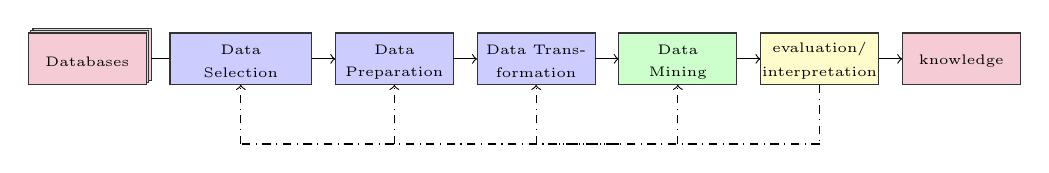
\begin{tikzpicture}[scale=0.6]
			\draw[draw, black!80, fill=blue!20!red!20] (-2.90,0.10) rectangle (-0.40,1.20);
			\draw[draw, black!80, fill=blue!20!red!20] (-2.95,0.05) rectangle (-.45,1.15);
			\draw[draw, black!80, fill=blue!20!red!20] (-3,0) rectangle (-0.5,1.1);
			\node (AMP) at (-1.75,0.5) {\tiny Databases};
			
			%\visible<2->
			{
				\draw[->] (-0.4,0.55)--(1.5,0.55);
				\draw[draw, black!80, fill=blue!20] (0,0) rectangle (3,1.1);
				\node (AMP) at (1.5,0.75) {\tiny Data};
				\node (AMP) at (1.5,0.25) {\tiny Selection};
			}
			
			%\visible<3->
			{
				\draw[->] (3,0.55)--(3.5,0.55);
				\draw[draw, black!80, fill=blue!20] (3.5,0) rectangle (6,1.1);
				\node (AMP) at (4.75,0.75) {\tiny Data};
				\node (AMP) at (4.75,0.25) {\tiny Preparation};
			}
			
			
			%\visible<4->
			{
				\draw[->] (6,0.55)--(6.5,0.55);
				\draw[draw, black!80, fill=blue!20] (6.5,0) rectangle (9,1.1);
				\node (AMP) at (7.75,0.75) {\tiny Data Trans-};
				\node (AMP) at (7.75,0.25) {\tiny formation};
			}
			
			%\visible<5->
			{
				\draw[dash dot,->] (10.75,-1.25)--(10.75,0);
				\draw[->] (9.0,0.55)--(9.5,0.55);
				\draw[draw, black!80, fill=green!20] (9.5,0) rectangle (12,1.1);
				\node (AMP) at (10.75,0.75) {\tiny Data};
				\node (AMP) at (10.75,0.25) {\tiny Mining};
			}
			
			{
				\draw[->] (12,0.55)--(12.5,0.55);
				\draw[draw, black!80, fill=yellow!20] (12.5,0) rectangle (15,1.1);
				\node (AMP) at (13.75,0.25) {\tiny interpretation};
				\node (AMP) at (13.75,0.75) {\tiny evaluation/};
			}
			
			\draw[->] (15,0.55)--(15.5,0.55);
			\draw[draw, black!80, fill=blue!20!red!20] (15.5,0) rectangle (18,1.1);
			\node (AMP) at (16.75,0.5) {\tiny knowledge};
			
			
			%\visible<8->
			{
				\draw[dash dot,-] (9.5,-1.25) -- (1.5,-1.25);
				\draw[dash dot,->] (1.5,-1.25)--(1.5,0);
			}
			
			%\visible<9->
			{
				\draw[dash dot,->] (4.75,-1.25)--(4.75,0);
				\draw[dash dot,->] (7.75,-1.25)--(7.75,0);
			}
			
			%\visible<2->
			{
				\draw[dash dot,-] (13.75,0)--(13.75,-1.25);
				\draw[dash dot,-] (13.75,-1.25) -- (8,-1.25);
				
			}
		\end{tikzpicture}
		\caption{KDD process according to \cite{Fayyad:1996} (own reduced representation based on \cite{Fayyad:1996})} 
		\label{KDDFayyad}
	\end{center}
\end{figure}



% \GRAPHICSC{1.0}{1.0}{BigData/KDD}



At the beginning of the KDD process there is always the available database from which the knowledge is to be gained. From this, the data to be used must be selected from one or more databases and the data must then be processed and prepared. Only then can the data be used for knowledge extraction with the help of data mining methods. After evaluation and possibly several runs through the various steps, the knowledge gained can finally be extracted and used in the application.

Fayyad further divides this process into nine sub-steps, some of which are not directly represented in Figure \ref{KDDFayyad}. These nine steps are described below.

\subsubsection{1. Domain Knowledge (Developing an Understanding of the Application Domain)}.

First, the domain of the application must be defined and understood. This includes the domain knowledge needed for the application to be able to perform the analysis in a way that leads to real added value. In addition, the precise objectives of the KDD process must be defined for the use case and the specific end user of the knowledge \cite{Fayyad:1996,Kurgan:2006}. This step forms the basis for making the decisions necessary in the next steps. 
necessary decisions in the next steps \cite{Maimon:2010}.

\subsubsection{2. Creating a Target Data Set}

Next, a data set or a subset of a data set is selected. Single or multiple variables can be selected to narrow down the data from which knowledge is to be extracted. \cite{Fayyad:1996} This involves determining what data is available and possibly obtaining any data that is still missing. It is important that all necessary information is included. Deciding which variables are necessary must be based on domain knowledge. After selecting the variables, as many representatives of the variables as possible should become available to the algorithm for a good model. On the other hand, the collection, storage and processing of larger data sets is more costly and many variables can also lead to results that are difficult to interpret. Therefore, the relevance of returning to steps that have already been carried out when gaining knowledge should already be seen in this step.\cite{Maimon:2010}

\subsubsection{3. Data Cleaning and Preprocessing}

This step aims to improve data reliability. This includes removing noise and outliers, but also dealing with missing data. If an attribute is not reliable enough, a data mining method can already be used at this point to improve the data.\cite{Maimon:2010} Time series information and known changes must also be taken into account. \cite{Kurgan:2006} Data cleaning and preparation is the most time-consuming step in the KDD process. Its share of the time to be spent on the KDD process is estimated by many sources to be about 60 \%.\cite{Kurgan:2006}

\subsubsection{4. Data Reduction and Transformation (Data Reduction and Projection)}.

To further improve the data, useful features are sought to represent the data \cite{Fayyad:1996}. Possible methods include dimensionality reduction and transformation. The implementation of this step will vary greatly depending on the application and domain. As in the previous steps, the most effective transformation may emerge during the KDD process \cite{Maimon:2010}. The importance of this step is made clearer by the application example in section~\ref{ExampleKDD}.

\subsubsection{5. Choosing the DM Task}

After the preparation of the data has been completed, a suitable data mining method is selected. Which method is suitable depends largely on the objectives defined in the first step \cite{Fayyad:1996}. A basic distinction is made between descriptive methods, which aim at interpreting and understanding the data, and predictive methods, which provide a behavioural model that is able to predict certain variables for previously unseen data. For this purpose, regressions can be used on the one hand, and classification methods such as decision trees, support vector machines or neural networks on the other. Some of these models can also be used for descriptive statements. \cite{Maimon:2010}

\subsubsection{6. Choosing the DM Algorithm}

In this step, the specific data mining algorithm to be used is selected. If, for example, it was decided in the previous step that a predictive method should be chosen, a choice must now be made between, for example, neural networks and decision trees, whereby the former provide more precise descriptions of the correlations, but the latter are easier to interpret. \cite{Maimon:2010}

\subsubsection{7. Data Mining}

In the seventh step, data mining is finally applied. Often data mining and KDD are used synonymously, but in fact data mining is a sub-step of the KDD process. \cite{Fayyad:1996}
This step may also have to be carried out several times, possibly even immediately one after the other, 
to optimise the hyperparameters. \cite{Maimon:2010}

\subsubsection{8. Interpreting the Results (Interpreting Mined Patterns)}

After the data mining has been successfully completed, the results are evaluated and interpreted. The visualisation of found patterns or models can be helpful for this. In this step, the influence of the data preparation steps is reflected on and possibly returned to. It must also be evaluated whether the model found is plausible and usable. \cite{Fayyad:1996,Maimon:2010}

\subsubsection{9. Applying the Results (Acting on Discovered Knowledge)}

The discovered knowledge can now be used. The product of this can be documentation or reports that record the knowledge obtained so that it can be used by interested parties. Furthermore, the extracted knowledge can be integrated into another system, e.g. in the form of a prediction model. By applying it under real conditions, e.g. with dynamic instead of static data, deficits can become apparent that still need to be reworked. \cite{Fayyad:1996,Maimon:2010}

\section{Generic Process Model}

Based on the models of Fayyad et al, Cabena et al, Cios et al and Anand \& Buchner and the CRISP-DM model, \cite{Kurgan:2006} describes a generic KDD model. This is structured very similarly to Fayyad's model described above and also runs through the steps iteratively. However, the steps are summarised differently, so that the model gets by with six instead of nine steps. 

\subsubsection{1. Application Domain Understanding}

As with Fayyad, the first step is to understand the application and objective as a prerequisite for the following steps.

\subsubsection{2. Understanding the Data (Data Understanding)}

The general understanding of the data corresponds roughly to the second step according to Fayyad. It involves looking at the available data set and identifying opportunities and problems.

\subsubsection{3. Data Preparation and Identification of DM Technology}

This step combines steps three to six according to Fayyad. This makes sense insofar as the type of data preparation and the data mining method to be applied influence each other and a clear separation is therefore difficult.


\subsubsection{4. Data Mining}

The data mining step as the core of the KDD process remains unchanged.

\subsubsection{5. Evaluation}

The generic model also emphasises the iterative nature of the KDD process. Therefore, an evaluation of the obtained results is indispensable.

\subsubsection{6. Knowledge Deployment (Knowledge Consolidation and Deployment)}

This step also hardly differs from the last process step according to Fayyad. The different models mainly differ in the way the discovered knowledge is used, which is due to the different application domains. While the models geared towards business applications mainly focus on reports and visualisation, the technical applications have a stronger emphasis on dynamic uses of created models.
\chapter{Applying of the Process to our project}
\label{KDDP}
The process we´re using in this project in also mainly based on the model of Fayyad.

\begin{figure}
	\centering
	
\includegraphics[width=1\textwidth]{images/KDD Process}
	\caption{KDD Process - Machine Learning Pipeline}
	\label{KDD Process}
	
\end{figure}

\section{Development}
\subsection{Data selection}
WISDM Dataset
\subsection{Data preparation}

\subsection{Data transformation}

\subsection{Data mining}

\subsection{Evaluation and verification}
\section{Deployment}
\subsection{Testing the Hardware}

\subsubsection{General Tests}

All the Arduino boards need power to operate, either it comes from the USB connection with Laptop, Ac power adapter, Battery or a regulated power supply. The most easiest way to operate arduino board is USB connection with laptop, normally these boards need 5V direct current (DC) to operate. Arduino Nano 33 BLE sense also need these types of power sources for funcnality, when applying one of the above mention power source the green LED glows as shown in the figure \ref{fig:Test}, it shows the sign of Arduino board working.

\begin{figure}[htbp]
	\centering
	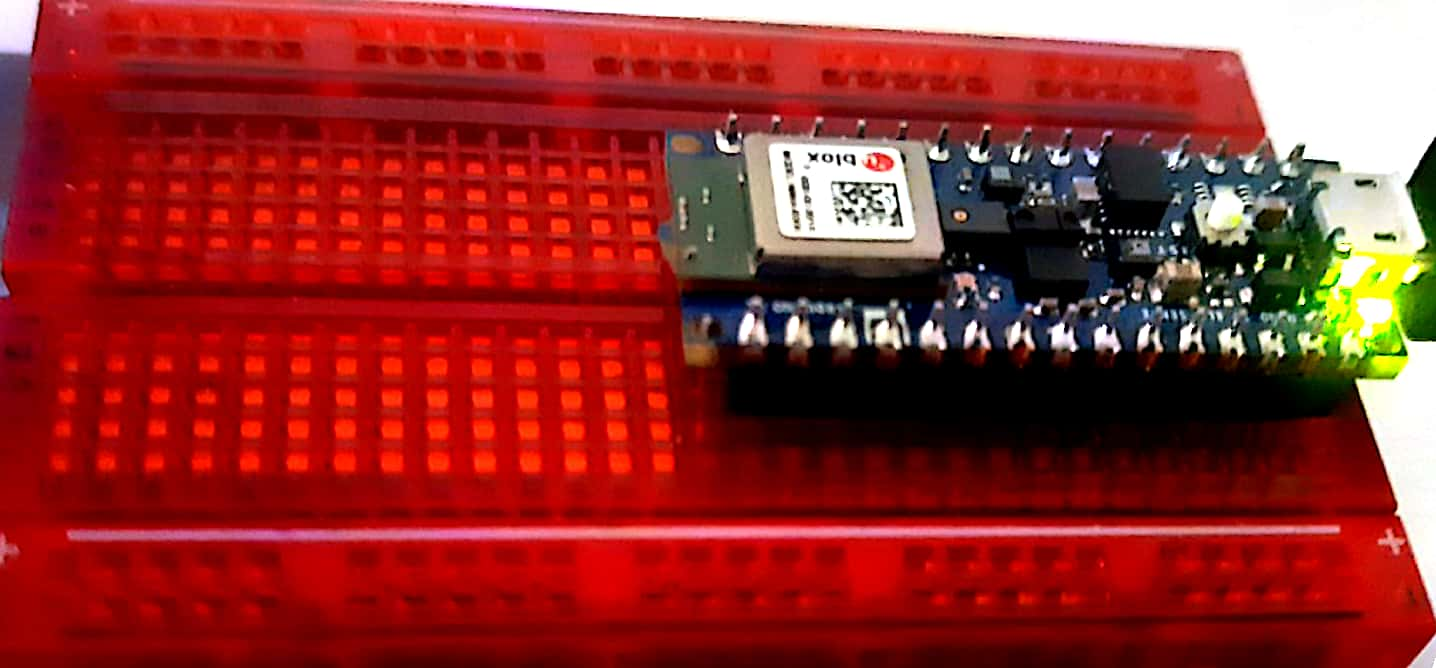
\includegraphics[width=6.5cm]{Images/Arduino/Test-1}
	\caption{Power On Arduino Nano 33 BLE Sense}
	\label{fig:Test}
\end{figure}

\paragraph{Test with Bluetooth Module Connection}

The same procedure we need to follow for making the successful bleutooth coonection, the one we follow for on-board sensors. Below figure \ref{fig:testsoftware-fur-bluetooth} shows the ArduinoBLE library in the example section of Arduino IDE.

\begin{figure}[h]
	\centering
	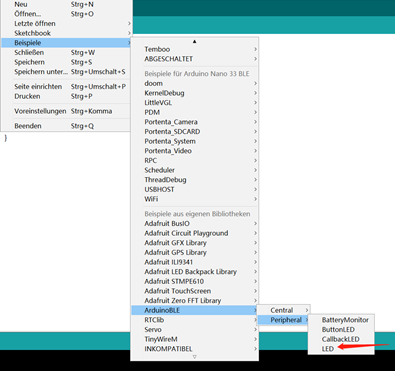
\includegraphics[width=0.7\linewidth]{Images/Arduino/TestsoftwareBluetooth}
	\caption{Bluetooth Connection}
	\label{fig:testsoftware-fur-bluetooth}
\end{figure}

Bluetooth wireless technology allows us to share the data, the voice, the music, the video, and a lot of information between paired devices, It is built into many products, from mobile phones, cars to medical devices and computers. It has lower power consumption. It is easily upgradeable. It has range better than Infrared communication. Bluetooth is used for voice and data transfer, we can communicate by recieving and sending the data with other bluetooth connected devices. It is also possible to output a value on the phone side or also on the laptop by making the proper pairing. 



\subsection{ML Pipeline}
\subsubsection{Using of TensorFlow}
TensorFlow: General, uses, user manual  

\subsubsection{Using Of TensorFlow Lite}
\subsubsection{Using Of TensorFlow Micro}
\subsubsection{Creating the Application with the Arduino IDE}


\subsection{Application "Recognizing Gait Patterns}
\subsubsection{Installation}
\subsubsection{Configuration}
\subsubsection{Tests}
\subsubsection{In the Field}
\subsection{Monitoring}
\chapter{Questions/To dos/ Conclusion}
\subsection{Appendix}
\subsubsection{Material List}
\subsubsection{Data sheets}


%\section{Introduction}
%A good database is important in order to achieve accurate gait detection since the model is trained on a particular set of data. 
%feeding our model a good and labeled Database will help detect recurring characteristics and features for each of the 4 modes (running, walking, jumping, and staying still) .this will register the pattern for each mode and permit comparison.
%“Knowledge Discovery in Databases (KDD) is the nontrivial
%process of identifying valid, novel, potentially useful, and ultimately
%understandable patterns in data”.
%[Fayyad, Piatetsky-Shapiro, and Smyth 1996]
%this project is based on data collected during the reasearch through the 9-axis inertial measurement unit (IMU) present on the Arduino board and will consist of the calculated thigh angle and the velocity.
%the data are saved in an excel sheet and transformed into line diagrams that can later be used to train the model.
%\section{Data selection}
%The data to be used can now be selected from the databases that have been identified, are available and can be used for the application. For example, a database could be used in its entirety, but only a part of such a database can be used or several databases can be combined. It is extremely important that all classes that are to be recognised are also present in the selected data. How many diagrams are selected depends on the planned scope of the training and the test, which has a significant influence on the training time, but possibly also on the performance of the model obtained. 
%\section{Data preparation}
%Data preprocessing is usually primarily concerned with data cleaning. This mainly includes the removal of outliers. In terms of tables, these outliers are mainly unlogical number or unexisting ones in certain cells. These should be removed or processed with suitable algorithms. 
%Furthermore, the data/diagrams must be converted into the format supported by the respective platform. It should be taken into account that compressed file formats cannot always be decompressed without loss.
%%\section{Preparation of Datasets for the Gait Patterns}
%\section{Data Transformation}
%
%\section{Data Mining}
%In the data mining step, the actual model building takes place. First, the algorithm must be chosen or the architecture defined and the model built accordingly. If deep learning algorithms are used, the architecture must be defined. With the definition of the architecture, the hyperparameters are determined.  Then the algorithm can be trained with the selected Data. During training, the weights are optimised. Their adjustment is done on the basis of the training data. After a given number of trainings, the validation data are used to test the accuracy of the current model. After several epochs, i.e. several runs of all training data, the model can be tested.
%\subsection {Convolutional Neural Networks (CNN)}
%the algorithm used is the Convolutional Neural Network (CNN) and is commonly used for image classification tasks.
%Convolutional Neural Networks (CNNs) are a type of neural network that are specifically designed to process data with a grid-like topology, such as an image. They are particularly well-suited for image classification tasks because they are able to automatically learn spatial hierarchies of features from input data, which is important for recognizing patterns and objects in images.
%CNNs have several key features that make them effective for image classification:\\
%
%Convolutional layers: These layers apply a convolution operation to the input data, which helps to extract features from the data by sliding a filter over it.\\
%
%Pooling layers: These layers down-sample the feature maps produced by the convolutional layers, which helps to reduce the computational burden and make the model more robust to small translations and deformations in the input data.\\
%
%Fully-connected layers: These layers perform classification by using the features extracted by the convolutional and pooling layers.
%
%%\subsection {Trenieren }
%%\subsection {Evaluierung und Verifikation}
%%\subsection{Training the Model}
%\section{Evaluation and Verification}
%
%In the first instance, the interpretation and evaluation of the trained model is done repeatedly during the training with the help of the validation data set. In the second instance, the model is tested directly after training with the help of the test images that are still unknown to the model. If the results are satisfactory, the model can be integrated into the application. In this instance, too, it is important to test the performance of the model in order to be able to draw conclusions and make corrections. In the dynamic application, other framework conditions prevail, so that drawing conclusions about necessary corrections in the previous steps may require great domain knowledge.
%
%The interpretation of the found model is not trivial for neural networks, especially for complex networks like \ac{cnn}. It may not be possible to extract direct correlations that could be transferred to other applications.
%%'\section{Quelle für die Datenbank}
%%- Format?
%%- extern oder intern ?
%
%%\section{Qualitätprufung}
%%\section{Zeitbereich und Format anpassen}
%\subsection{Model}
%The trained model can finally be integrated into the intended application. While the data preparation and training take place on a computer that is generally equipped with high computing power, the model is intended to be used on a microcontroller. Motion recognition could be performed based on the training with the static images/Line diagrams. Transferring the model to the micro-computer may require converting the model to a different format due to the lack of memory.
%


